\documentclass[12pt,amstags,fleqn]{article}

% Uncomment only one of these lines:
%\usepackage[mathlf,textlf,minionint]{MinionPro} \usepackage[T1]{fontenc} \usepackage{textcomp} \usepackage{amsthm}
\usepackage{amssymb}

\usepackage{url}

\usepackage{xspace}

\usepackage{fancyvrb}
\usepackage{color}
\usepackage{fancyvrb}
\usepackage{color}

\newcommand\at{@}
\newcommand\lb{[}
\newcommand\rb{]}
\newcommand\PYbg[1]{\textcolor[rgb]{0.00,0.50,0.00}{\textbf{#1}}}
\newcommand\PYbf[1]{\textcolor[rgb]{0.73,0.40,0.53}{\textbf{#1}}}
\newcommand\PYbe[1]{\textcolor[rgb]{0.40,0.40,0.40}{#1}}
\newcommand\PYbd[1]{\textcolor[rgb]{0.73,0.13,0.13}{#1}}
\newcommand\PYbc[1]{\textcolor[rgb]{0.00,0.50,0.00}{\textbf{#1}}}
\newcommand\PYbb[1]{\textcolor[rgb]{0.40,0.40,0.40}{#1}}
\newcommand\PYba[1]{\textcolor[rgb]{0.00,0.00,0.50}{\textbf{#1}}}
\newcommand\PYaJ[1]{\textcolor[rgb]{0.73,0.13,0.13}{#1}}
\newcommand\PYaK[1]{\textcolor[rgb]{0.00,0.00,1.00}{#1}}
\newcommand\PYaH[1]{\fcolorbox[rgb]{1.00,0.00,0.00}{1,1,1}{#1}}
\newcommand\PYaI[1]{\textcolor[rgb]{0.69,0.00,0.25}{#1}}
\newcommand\PYaN[1]{\textcolor[rgb]{0.00,0.00,1.00}{\textbf{#1}}}
\newcommand\PYaO[1]{\textcolor[rgb]{0.00,0.00,0.50}{\textbf{#1}}}
\newcommand\PYaL[1]{\textcolor[rgb]{0.73,0.73,0.73}{#1}}
\newcommand\PYaM[1]{\textcolor[rgb]{0.74,0.48,0.00}{#1}}
\newcommand\PYaB[1]{\textcolor[rgb]{0.00,0.25,0.82}{#1}}
\newcommand\PYaC[1]{\textcolor[rgb]{0.67,0.13,1.00}{#1}}
\newcommand\PYaA[1]{\textcolor[rgb]{0.00,0.50,0.00}{#1}}
\newcommand\PYaF[1]{\textcolor[rgb]{1.00,0.00,0.00}{#1}}
\newcommand\PYaG[1]{\textcolor[rgb]{0.10,0.09,0.49}{#1}}
\newcommand\PYaD[1]{\textcolor[rgb]{0.25,0.50,0.50}{\textit{#1}}}
\newcommand\PYaE[1]{\textcolor[rgb]{0.63,0.00,0.00}{#1}}
\newcommand\PYaZ[1]{\textcolor[rgb]{0.00,0.50,0.00}{\textbf{#1}}}
\newcommand\PYaX[1]{\textcolor[rgb]{0.00,0.50,0.00}{#1}}
\newcommand\PYaY[1]{\textcolor[rgb]{0.73,0.13,0.13}{#1}}
\newcommand\PYaR[1]{\textcolor[rgb]{0.10,0.09,0.49}{#1}}
\newcommand\PYaS[1]{\textcolor[rgb]{0.25,0.50,0.50}{\textit{#1}}}
\newcommand\PYaP[1]{\textcolor[rgb]{0.49,0.56,0.16}{#1}}
\newcommand\PYaQ[1]{\textcolor[rgb]{0.40,0.40,0.40}{#1}}
\newcommand\PYaV[1]{\textcolor[rgb]{0.00,0.00,1.00}{\textbf{#1}}}
\newcommand\PYaW[1]{\textcolor[rgb]{0.73,0.13,0.13}{#1}}
\newcommand\PYaT[1]{\textcolor[rgb]{0.50,0.00,0.50}{\textbf{#1}}}
\newcommand\PYaU[1]{\textcolor[rgb]{0.82,0.25,0.23}{\textbf{#1}}}
\newcommand\PYaj[1]{\textcolor[rgb]{0.00,0.50,0.00}{#1}}
\newcommand\PYak[1]{\textcolor[rgb]{0.73,0.40,0.53}{#1}}
\newcommand\PYah[1]{\textcolor[rgb]{0.63,0.63,0.00}{#1}}
\newcommand\PYai[1]{\textcolor[rgb]{0.10,0.09,0.49}{#1}}
\newcommand\PYan[1]{\textcolor[rgb]{0.67,0.13,1.00}{\textbf{#1}}}
\newcommand\PYao[1]{\textcolor[rgb]{0.73,0.40,0.13}{\textbf{#1}}}
\newcommand\PYal[1]{\textcolor[rgb]{0.25,0.50,0.50}{\textit{#1}}}
\newcommand\PYam[1]{\textbf{#1}}
\newcommand\PYab[1]{\textit{#1}}
\newcommand\PYac[1]{\textcolor[rgb]{0.73,0.13,0.13}{#1}}
\newcommand\PYaa[1]{\textcolor[rgb]{0.50,0.50,0.50}{#1}}
\newcommand\PYaf[1]{\textcolor[rgb]{0.25,0.50,0.50}{\textit{#1}}}
\newcommand\PYag[1]{\textcolor[rgb]{0.40,0.40,0.40}{#1}}
\newcommand\PYad[1]{\textcolor[rgb]{0.73,0.13,0.13}{#1}}
\newcommand\PYae[1]{\textcolor[rgb]{0.40,0.40,0.40}{#1}}
\newcommand\PYaz[1]{\textcolor[rgb]{0.00,0.63,0.00}{#1}}
\newcommand\PYax[1]{\textcolor[rgb]{0.60,0.60,0.60}{\textbf{#1}}}
\newcommand\PYay[1]{\textcolor[rgb]{0.00,0.50,0.00}{\textbf{#1}}}
\newcommand\PYar[1]{\textcolor[rgb]{0.10,0.09,0.49}{#1}}
\newcommand\PYas[1]{\textcolor[rgb]{0.73,0.13,0.13}{\textit{#1}}}
\newcommand\PYap[1]{\textcolor[rgb]{0.00,0.50,0.00}{#1}}
\newcommand\PYaq[1]{\textcolor[rgb]{0.53,0.00,0.00}{#1}}
\newcommand\PYav[1]{\textcolor[rgb]{0.00,0.50,0.00}{\textbf{#1}}}
\newcommand\PYaw[1]{\textcolor[rgb]{0.40,0.40,0.40}{#1}}
\newcommand\PYat[1]{\textcolor[rgb]{0.10,0.09,0.49}{#1}}
\newcommand\PYau[1]{\textcolor[rgb]{0.40,0.40,0.40}{#1}}


\usepackage{amsmath}
\usepackage{amsthm}

\theoremstyle{plain}
\newtheorem{theorem}{Theorem}[section]
\newtheorem{lemma}[theorem]{Lemma}
\newtheorem{proposition}[theorem]{Proposition}
\newtheorem{corollary}[theorem]{Corollary}
\newtheorem{conjecture}[theorem]{Conjecture}

\theoremstyle{definition}
\newtheorem{definition}[theorem]{Definition}
\newtheorem{construction}[theorem]{Construction}
\newtheorem{convention}[theorem]{Convention}


% CH: I like Remarks to be in normal font, not italics.
\theoremstyle{definition}
\newtheorem{example}[theorem]{Example}
\newtheorem{remark}[theorem]{Remark}
\newtheorem{question}[theorem]{Question}

%%%%%%%%%%%%%%%%%%%%%%%%%%%%%%%%%%%%%%%%%%%%%%%%%%%%%%%%%%
% This stuff is needed to correctly render the metapost
% diagrams depending on whether latex or pdflatex was
% called. Don't change any of it!
\usepackage{ifpdf}

\ifpdf
        \pdfcompresslevel=9
        \usepackage[pdftex]{graphicx}
        %\usepackage{thumbpdf}
        \usepackage[pdftex,colorlinks,bookmarks,backref]{hyperref}
        %\usepackage[pdftex,backref]{hyperref}
        \DeclareGraphicsRule{*}{mps}{*}{}
\else
        %\usepackage{hyperref}
        %\usepackage[dvips]{graphicx}
        %\usepackage[dvips]{color}
    \usepackage{epsfig}
        \usepackage{graphicx}
        \DeclareGraphicsRule{*}{eps}{*}{}
\fi
%%%%%%%%%%%%%%%%%%%%%%%%%%%%%%%%%%%%%%%%%%%%%%%%%%%%%%%%%%



\title{Gibbs Sampling}

\author{Carlo H\"{a}m\"{a}l\"{a}inen\\
{\texttt{carlo.hamalainen@gmail.com}}}

%\date{}

\begin{document}

\maketitle

This file and related Sage source code is available at
\url{http://carlo-hamalainen.net/stuff/gibbs} \\

Suppose that $X$ and $Y$ are two random variables. The Gibbs sampling
algorithm gives us a way to sample from $f(x)$ by sampling from the
conditional distributions $f(x \mid y)$ and $f(y \mid x)$. In
statistical models we often know the conditional distribution while the
marginal distribution $f(x)$ is difficult to compute.

In Gibbs sampling we generate a series of random variables
\[
Y'_0, X'_0,
Y'_1, X'_1,
Y'_2, X'_2,
\dots
Y'_k, X'_k
\]
where $Y'_0 = y_0$ is fixed and the rest of the variables are sampled
according to
\begin{align*}
X'_j &\sim f(x \mid Y'_j = y'_j) \\
Y'_{j+1} &\sim f(y \mid X'_j = x'_j).
\end{align*}
If $k$ is large enough then $X'_k$ will effectively be a sample from the
marginal distribution $f(x)$.

We can work through the two variable case with an explicit example,
following~\cite{gibbs}. Let $X$ and $Y$ each be (marginally) Bernoulli
random variables with joint distribution as follows:

\begin{center}  
\begin{tabular}{|c|c|c|}
\hline ~ & $X=0$ & $X=1$ \\
\hline $Y=0$ & $p_1$ & $p_2$ \\
\hline $Y=1$ & $p_3$ & $p_4$ \\
\hline
\end{tabular}
\end{center}
where $0 \leq p_i \leq 1$ and $\sum_i p_i = 1$. Using this table we can
calculate the conditional distributions. For example,
\begin{align*}
P(X = 1 \mid Y = 1) &= \frac{P(X = 1 \textnormal{ and } Y = 1)}{P(Y = 1)}
= p_4/(p_3 + p_4).
\end{align*}
The matrix $A_{y\mid x}$ gives the conditional probability of $Y$ given $X = x$:
\[
A_{y \mid x} = 
\left(\begin{array}{rr}
\frac{p_{1}}{{(p_{1} + p_{3})}} & \frac{p_{3}}{{(p_{1} + p_{3})}} \\
\frac{p_{2}}{{(p_{2} + p_{4})}} & \frac{p_{4}}{{(p_{2} + p_{4})}}
\end{array}\right)
\]
The matrix $A_{x\mid y}$ gives the conditional probability of $X$ given $Y = y$:
\[
A_{x \mid y} = 
\left(\begin{array}{rr}
\frac{p_{1}}{{(p_{1} + p_{2})}} & \frac{p_{2}}{{(p_{1} + p_{2})}} \\
\frac{p_{3}}{{(p_{3} + p_{4})}} & \frac{p_{4}}{{(p_{3} + p_{4})}}
\end{array}\right)
\]
The transition $X'_0 \rightarrow Y'_1 \rightarrow X'_1$ has probability
\[
P(X'_1 = x_1 \mid X'_0 = x_0)
= \sum_{y}P(X'_1 = x_1 \mid Y'_1 = y)
P(Y'_1 = y \mid X'_0 = x_0).
\]
So the matrix $A_{x\mid x}$ describing the transitions 
$X'_0 \rightarrow X'_1$ is
\[
A = A_{x\mid x} = A_{y \mid x} A_{x \mid y} = \left(\begin{array}{rr}
\frac{p_{3}^{2}}{{(p_{3} + p_{4})} {(p_{1} + p_{3})}} +
\frac{p_{1}^{2}}{{(p_{1} + p_{3})} {(p_{1} + p_{2})}} & \frac{p_{3}
p_{4}}{{(p_{3} + p_{4})} {(p_{1} + p_{3})}} + \frac{p_{1} p_{2}}{{(p_{1}
+ p_{3})} {(p_{1} + p_{2})}} \\
\frac{p_{3} p_{4}}{{(p_{3} + p_{4})} {(p_{2} + p_{4})}} + \frac{p_{1}
p_{2}}{{(p_{2} + p_{4})} {(p_{1} + p_{2})}} &
\frac{p_{4}^{2}}{{(p_{3} + p_{4})} {(p_{2} + p_{4})}} +
\frac{p_{2}^{2}}{{(p_{2} + p_{4})} {(p_{1} + p_{2})}}.
\end{array}\right)
\]
We now have a Markov chain with two states, $0$ and $1$, and transition
probabilities given by the matrix $A$. Note that
$A_{0,0} + A_{0,1} = 1$ and
$A_{1,0} + A_{1,1} = 1$ since $A$ is a stochastic matrix.

The stationary distribution is given by the normalised eigenvector $f$,
where $fA = f$. For our the $2 \times 2$ case the $f$ vector is:
\[
f = 
\left(\begin{array}{rr}
\frac{{(\frac{{(p_{2} + p_{4})} p_{1}}{{(p_{1} + p_{2} + p_{3} +
p_{4})}} + \frac{{(p_{2} + p_{4})} p_{3}}{{(p_{1} + p_{2} + p_{3} +
p_{4})}})}}{{(p_{2} + p_{4})}} & \frac{{(p_{2} + p_{4})}}{{(p_{1} +
p_{2} + p_{3} + p_{4})}}
\end{array}\right)
\]
Observe that $f$ is undefined if $p_2 + p_4 = 0$. In terms of the
original joint distribution, this means that there is zero probability
of reaching a state $(1, Y)$ for any $Y$. So this case is in some sense
degenerate.

For an explicit example, set
\begin{align*}
p_1 &= 0.26275562241164158 \\
p_2 &= 0.6960509654605056 \\
p_3 &= 0.025834046671036285 \\
p_4 &= 0.015359365456816687
\end{align*}
Then 
\[
A = \left(\begin{array}{rr}
0.305652971862979 & 0.694347028137022 \\
0.281667794759494 & 0.718332205240506
\end{array}\right)
\]
and
\[
f = \left(\begin{array}{rr}
0.288589669082678 & 0.711410330917322
\end{array}\right)
\]
The error in the stationary distribution of $X=1$ is given in the
following plot:
\begin{center}
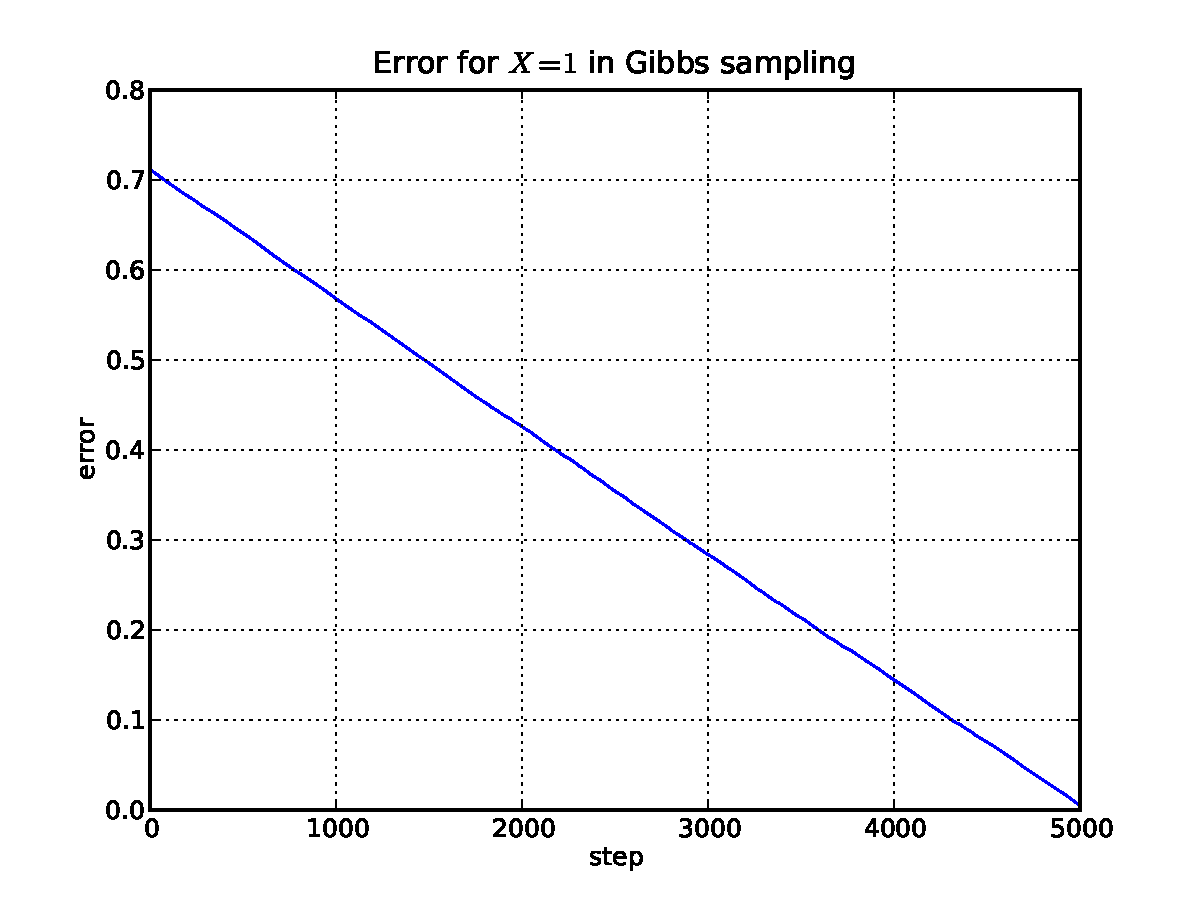
\includegraphics[width=.75\textwidth]{gibbs_2x2_error.pdf}
\end{center}
With the same matrices, we can also compare the error in the $X=1$
stationary probability, starting from an initial distribution of $f_0 =
[0.5 \,\,\, 0.5]$: 
\begin{center}
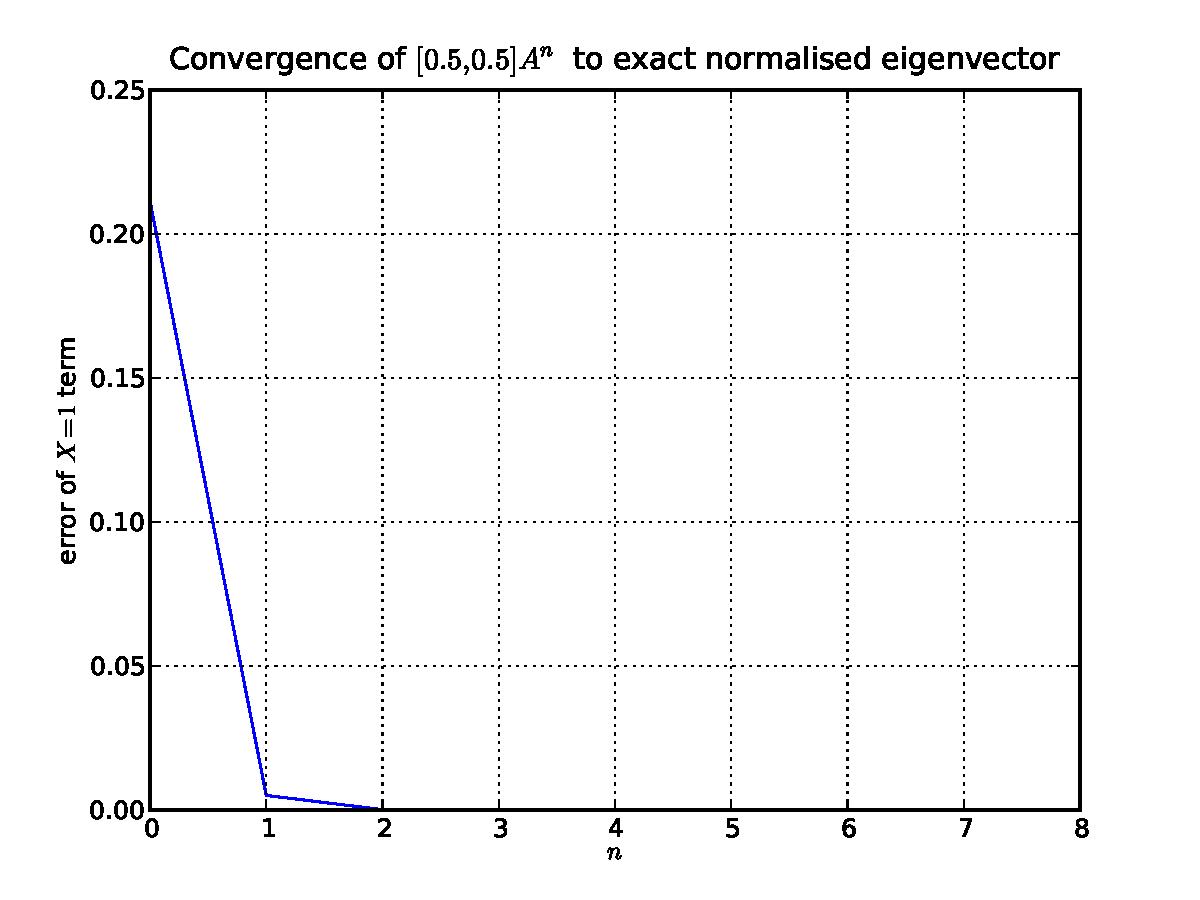
\includegraphics[width=.75\textwidth]{gibbs_error_matrix_mult.pdf}
\end{center}

\bibliographystyle{plain}
\bibliography{gibbs}

\end{document}
